\documentclass[a4paper]{article}
\usepackage{exercise}

\renewcommand{\title}{Aufgabenseminar\\ Mathematische Methoden}
\newcommand{\titleh}{Aufgabenseminar Mathematische Methoden}

%\usepackage{exercise} 
\usepackage{../images/preamble}
\usepackage{rotating}
\usetikzlibrary{decorations.pathmorphing}
\usetikzlibrary{decorations.markings}
\usetikzlibrary{arrows}
\usetikzlibrary{shapes.geometric}
\usepackage{mathrsfs}
\newcommand{\midarrow}{\tikz \draw[-triangle 90] (0,0) -- +(.02,0);}
\usepackage{xcolor}
%\usepackage{draftwatermark}
%\SetWatermarkText{\textsc{Entwurf}}
%\SetWatermarkScale{6}
%\SetWatermarkColor{red!30}

 
\fancyhead[L]{
\includegraphics[width=2cm]{../images/logo_scaled.pdf}}
\fancyhead[R]{\textsc{\titleh}}



\begin{document}
	\vspace*{-1cm}
	\parbox{4cm}{\vspace{-0.2cm}
\includegraphics[width=5cm]{../images/logo_scaled.pdf}}
	\parbox{10.6cm}{\setstretch{2.0} \centering{ \huge \textsf{\title
			}}\\\url{pankratius.github.io/rolf}
			 }
		\vspace{0.5cm}
	
\thispagestyle{empty}


\noindent




\begin{Exercise}[label = moveant, origin = {Jaan Kalda,\url{http://www.ioc.ee/~kalda/ipho/}}, difficulty = 3, title = Ameise auf dem Laufband]
	Eine Ameise bewegt sich auf einem Gummiband der Länge $\ell_0$ mit einer Geschwindigkeit $v$. Das Ende des Gummibands, an dem die Ameise startet, ist fest mit einer Wand verbunden. An dem anderen Ende zieht man so, dass sich die Länge des Bandes mit einer Geschwindigkeit $u$ ändert. Wie lange braucht die Ameise, um das andere Ende des Bandes zu erreichen? Was passiert für $v=u$?
\end{Exercise}
\begin{Answer}[ref = moveant]
	Die Gesamtgeschwindigkeit der Ameise setzt sich zusammen aus der durch ihre eigene Bewegung, also $v$, und der Geschwindigkeit der Ausdehnung des Gummibands.\\
	Wenn sich die Gesamtlänge des Gummibandes mit der Geschwindigkeit $u$ ändern soll, folgt aus dem Hookschen Gesetz, dass die Änderungsrate der Gummibandlänge an einer Position $x$ proportional zu dieser ist. Das heißt einfach nur, dass sich das Gummiband an der Stelle $x$ mit der Geschwindigkeit $v_gu = u \frac{x}{\ell\left(t\right)}$ bewegt. Hierbei müssen wir beachten, dass natürlich die Länge des Gummibandes zum aktuellen Zeitpunkt relevant ist. Aus der Aufgabenstellung wissen wir aber, dass $\ell\left(t\right) = \ell_0 + v t $ ist. \\
	Mit all diesen Überlegungen kommen wir also auf eine Gesamtgeschwindigkeit $v_g$ der Ameise, die 
	\begin{equation}\label{moveant1:eom1}
	v_g = 	\underbrace{v}_{\mathrm{Ameisengeschwindigkeit}} +\underbrace{u\cdot \frac{x}{\ell_0 + u t}}_{Gummibandgeschwindigkeit}
	\end{equation}
	beträgt.\\
	Diese Gesamtgeschwindigkeit $v_g$ ist aber gerade die Änderungsrate der Ameisenposition, also die Ableitung der Ameisenposition $x$ nach der Zeit; $v_g = \dot{x}\left(t\right)$. Damit handelt es sich bei \eqref{moveant1:eom1} um eine sog. Differentialgleichung. Das heißt, dass sie die Ableitung einer Größe (die Ameisengeschwindigkeit als Funktion der Zeit) mit der Größe selbst (also der Ameisenposition als Funktion der Zeit) in Verbindung setzt. Wir können jetzt versuchen, die zu lösen.\\
	Das ist gar nicht \textit{so} einfach, weil es sich um eine sog. inhomogene Gleichung handelt. Das liegt daran, dass in \eqref{moveant1:eom1} nicht nur $x\left(t\right)$ und zeitliche Ableitungen davon auftreten, sondern auch das konstante Glied der Ameisengeschwindigkeit ($+v$).\\
	Eine solche inhomogene Gleichung löst man, indem man zuerst die homogene Variante davon betrachtet, und die löst. Die homogene Variante ist einfach die inhomogene Variante, ohne das konstante Glied:
	\begin{equation}\label{moveant1:hom}
		\dot{x}\left(t\right) = u\cdot \frac{x\left(t\right)}{\ell_0 + u t}.
	\end{equation}
	Die können wir lösen, indem wir einfach $\dot{x}\left(t\right)$ als $\frac{dx}{dt}$ schreiben, und dann so \glqq umstellen\grqq, dass wir gut integrieren können \footnote{Das ganze heißt eigentlich \textit{Separation der Variablen}. Und ja, umstellen darf man eigentlich immer bei solche Sachen!}. Dann kommen wir auf
	\begin{equation*}
		\frac{1}{x}~dx = \frac{u}{\ell_0 + u t}~dt
	\end{equation*}
	Hier können wir einfach integrieren, dürfen dabei aber die Integrationskonstante nicht vergessen:
	\begin{equation}\label{moveant1:homint}
		\int \frac{1}{x}~dx = \int \frac{u}{\ell_0+ut}~dt \Rightarrow \ln x = \ln \left(\ell_0 + ut\right) +c \Rightarrow x = a \left(\ell_0 + u t\right),
	\end{equation}
	wobei auch $a$ eine Konstante ist.\\
	Jetzt haben wir eine Lösung! Toll, nicht?\\
	Blöd ist nur, dass wir ja nur \eqref{moveant1:hom} gelöst haben. Das war aber eine ganz andere Gleichung. Der Trick beim Lösen solcher inhomogener Gleichungen ist jetzt, dass man $a$ nicht mehr konstant lässt. Vielmehr fragt man sich, ob es eine zeitabhängige Funkion $b\left(t\right)$ gibt, die man statt des konstanten $a$ an das Ergebnis aus \eqref{moveant1:homint} multipliziert, sodass man damit aber die inhomogene Variante, also \eqref{moveant1:eom1}, löst.\\
	Warum das funktioniert, werden wir gleich sehen.\\
	Um dieses neue $b\left(t\right)$ jetzt zu finden, setzten wir einfach für $x$ in \eqref{moveant1:eom1} $x\left(t\right) = b\left(t\right) \left(\ell_0 + u t\right) $ ein. Dafür brauchen wir aber noch $v_g$, also $\dot{x}\left(t\right)$. Das kriegen wir einfach mit der Produktregel
	\begin{equation}\label{moveant1:prodrule}
		\frac{d}{dt}\left(b\left(t\right)\cdot\left(\ell_0 + u t\right)\right) = \dot{b} \left(t\right)\cdot  \left(\ell_0 + u t\right)  + b\left(t\right)  \cdot u.
	\end{equation}
	Einsetzen in \eqref{moveant1:eom1} führt auf
	\begin{equation}\label{moveant1:homsub}
		\dot{b}\left(t\right) \cdot \left(\ell_0 + u t\right)  + b\left(t\right)  \cdot u = v + u\cdot \frac{b\left(t\right) \cdot \left(\ell_0 + u t\right)}{ \left(\ell_0 + u t\right)} = v + u b\left(t\right),
	\end{equation}
	weil wir im letzten Bruch kürzen durften. Jetzt steht aber sowohl links als auch rechts vom Gleichheitszeichen noch der Ausdruck $b\left(t\right)\cdot u$, denn wir einfach wegsubtrahieren können. Wenn wir das machen, kommen wir auf eine ganz einfache Gleichung für die Ableitung von $b\left(t\right)$, nämlich
	\begin{equation*}
		\dot{b}\left(t\right)\cdot \left(\ell_0 + u t\right) = v.
	\end{equation*}
	Die können wir wieder integrieren - Integrationskonstante nicht vergessen!
	\begin{equation}
	\int db = \int \frac{v}{\ell_0 + u t}~dt \Rightarrow b = \frac{v}{u}\cdot \ln \left(\ell_0 + u t\right)+c.
	\end{equation}
	Das ist die Form, die $b\left(t\right)$ haben muss, damit \eqref{moveant1:homint} eine Lösung von \eqref{moveant1:eom1} ist.\\
	Setzen wir ein, bekommen wir
	\begin{equation}\label{moveant1:homsolc}
		x\left(t\right) = \left( \frac{v}{u}\cdot \ln \left(\ell_0 + u t\right)+c\right) \cdot \left(\ell_0 + ut\right).
	\end{equation}
	Die Integrationskonstante $c$ finden wir, wenn wir eine $x$-Wert zu einem $t$-Wert kennen. Das tun wir. Weil die Ameise am Anfang, also bei $t=0$, am Ende des Gummis starten soll, ist $x\left(0\right) = 0$. Jetzt können wir einfach in \eqref{moveant1:homsolc} einsetzten, und nach $c$ umstellen
	\begin{equation*}
		0 = \left( \frac{v}{u}\cdot \ln \left(\ell_0 + u 0\right)+c\right) \cdot \left(\ell_0 + u 0\right) \Rightarrow c = - \frac{v}{u}\ln \ell_0.
	\end{equation*}
	Damit ist die fertige Lösung
	\begin{equation}
		x\left(t\right) = \frac{\left(\ell_0 + u t\right)v}{u}\cdot \left(\ln\left(\ell_0 + u t\right) - \ln \ell_0\right).
	\end{equation}
	Nun hat die Ameise das Band erreicht, wenn sie an der Position des Bandes ist, an der auch das Bandende ist, also $x\left(T\right) = \ell_0 + u T$. Damit kommen wir auf eine Gleichung, die die Kriechzeit $T$ bestimmt:
	\begin{equation}\label{moveant1:eom1sol}
	\boxed{
		\frac{u}{v} + \ln \ell_0 = \ln\left(\ell_0 + u t\right) \Rightarrow T = \frac{\ell_0}{u}\left(e^{\nicefrac{u}{v}}-1\right).}
	\end{equation}
	Ein bisschen einfacher kann man die Aufgabe auch lösen, wenn man ein bisschen nachdenkt. Dafür nehmen wir ein fancy Koordinatensystem, dass die Position der Ameise relativ zur Bandlänge angibt. Wir nennen diese Koordinate $\psi$. Befindet sich die Ameise am festen Ende des Bandes, also ganz am Anfang bei $t=0$, soll $\psi = 0$ gelten. Ist die Ameise am Ende angekommen, also bei $t=T$, soll $\psi  = 1$ sein (sog. Langrangsche Koordinaten). Allgemein ist also $\psi = \frac{x\left(t\right)}{\ell_0 + ut}$. In diesem mitbewegten Koordinatensyste wird auch die Geschwindigkeit der Ameise einfach mit $\frac{1}{\ell_0 + ut}$ skaliert, sodass wir als neue Bewegungsgleichung
	\begin{equation}\label{moveant1:eom2}
		\dot{\psi}\left(t\right) = \frac{v}{\ell_0 + ut}
	\end{equation}
	haben. Das ist im Gegensatz zu \eqref{moveant1:eom1} nicht mehr inhomogen, kann also einfach integriert werden
	\begin{equation*}
		\int~d\psi  = \int \frac{v}{\ell_0 + u t}~dt \Rightarrow \psi\left(t\right)= \frac{v}{u}\left(\ell_0 + ut\right) + c,
	\end{equation*}
	wobei $c$ schon wieder die Integrationskonstante ist.\\
	Weil wir festgelegt haben, dass $\psi\left(0\right) = 0$ ist, können wir $c$ wieder zu $c = -\frac{v}{u}\ln \ell_0$ bestimmen.\\
	Die Kriechzeit kriegen wir jetzt, indem wir uns einfach erinnern, dass am Ende $\psi\left(T\right) = 1$ gelten soll,
	\begin{equation}\label{moveant1:eom2sol}
	\boxed{
		1 = \frac{v}{u}\ln\left(\frac{\ell_0 + u T}{\ell_0}\right) \Rightarrow T = \frac{\ell_0}{u}\left(e^{\nicefrac{u}{v}}-1\right).} 
	\end{equation}
	Es kommt also bei beiden Gleichungen genau das selbe raus!
\end{Answer}
\begin{Exercise}[label = halfplan, title = Ein halber Planet, origin = {4.Runde IPhO 2015, Kurzaufgabe}, difficulty = 3]
	Auf einem halbkugelförmigen Planeten beträgt die Schwerebeschleunigung direkt in der Mitte der flachen Deckfläche $g_0$.  Die Dichte ist im gesamten Planeten gleich, und beträgt $\rho$. Wie groß ist der Planetenradius?
\end{Exercise}
\begin{Exercise}[label = boatgraph, origin = Jaan Kalda, difficulty = 4, title = Bootsbewegung]
	Die Beschleunigung eines Boots hängt von seiner Geschwindigkeit ab, wie im Bild gezeigt. Die Anfangsgeschwindigkeit des Bootes beträgt $v_0 = 4~\nicefrac{m}{s}$. Wie groß ist die Strecke, die das Boot zurücklegt hat, wenn es nahezu zum stehen kommt?
\end{Exercise}
\begin{figure}[h]
	\centering
	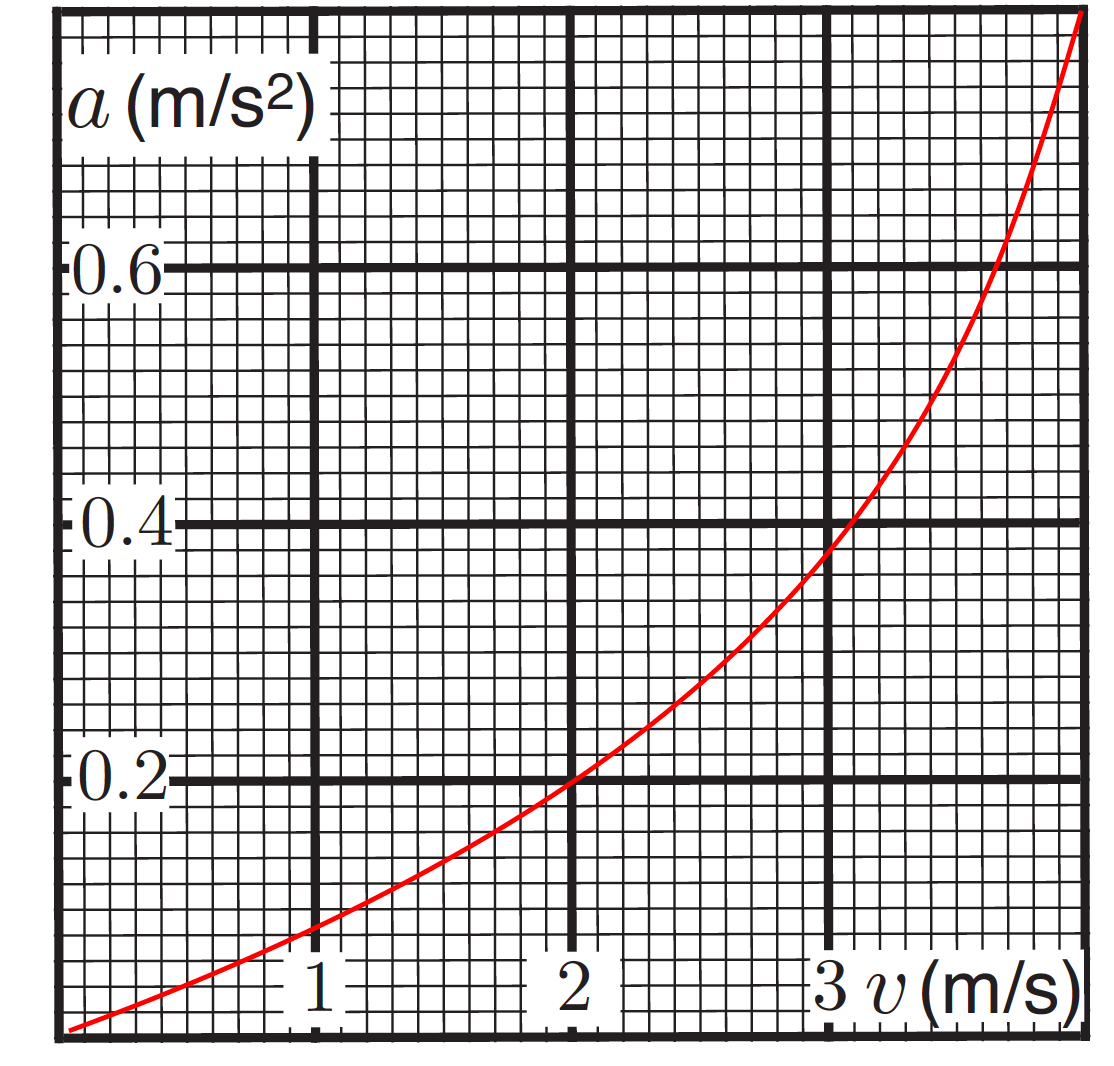
\includegraphics[scale = 0.4]{../tasks/kalda/boatgraph1}
\end{figure}
\begin{Exercise}[ref = cristall, title = Relexion im Kristall, dificulty = 3, origin = Aaron Wild]
	Betrachte einen Kristall, in dem aus irgendeinem Grund Licht entsteht.\\

\end{Exercise}
\begin{tikzpicture}
\filldraw[fill=grey!40!white, draw=black] (0,0) rectanlge (2,2);
\end{tikzpicture}
\begin{Exercise}[label = ants, difficulty = 3, title = Ameisen im Dreieck]
	Drei Ameisen sitzten an den Eckpunkten eines gleichseiten Dreiecks. Jede Ameise bewegt sich direkt auf ihren jeweils rechten Nachbarn mit der Geschwindigkeit $v$ zu. Stelle eine Gleichung der Form $r = f\left(\varphi\right)$ auf, die den Abstand $r$ einer Ameise vom Treffpunkt der drei in Abhängigkeit eines \textit{sinnvoll} definierten Winkels $\varphi$ angibt.
\end{Exercise}
\begin{Exercise}[label = devsandints, title = Ableit - und Integrierspaß]
	\Question
	Welche Ableitung haben folgende Funktionen?
	\begin{multicols}{3}
		\begin{enumerate}[(i)]
			\item $f_1(x) = 3$
 			\item $f_2(x)= \nicefrac{x^3}{3}$
			\item $f_3(x) = \exp x + \frac{3}{4}$
			\item $f_4(x) = \sin(x)\cdot\cos(x)$
			\item $f_5(x) = \exp(-\lambda\cdot \sqrt[3]{x^4})$
			\item $f_6(x) = \frac{x^2-16x+3}{\sin\left(\cos\left(x\right)\right)}$
			\item $f_7(x) = x^x$
			\item $f_8(x) = x^{\sqrt{x}}$
			\item $f_9(x) = \arcsin{x}$
		\end{enumerate}
	\end{multicols}
	\Question
	Welche Stammfunktionen haben folgende Funktionen?
	\begin{multicols}{3}
		\begin{enumerate}[(i)]
			\item $f_1 = 3$
			\item $f_2 = \frac{x^4}{9}$
			\item $f_3 = \lambda \exp(x)$
			\item $f_4 = \sin\left(x\right)$
			\item $f_5 = -\frac{19}{x^2}$
			\item $f_6 = -\frac{19}{x}$
			\item $f_7 = \frac{1}{\sqrt{1-x^2}}$
			\item $f_8 = 1+x^2$
			\item $f_9 = \sqrt{1-x^2}$
			
		\end{enumerate}
	\end{multicols}
\end{Exercise}

\end{document}
